% Created 2021-11-17 Wed 16:44
% Intended LaTeX compiler: xelatex
\documentclass[a4paper]{article}
\usepackage{graphicx}
\usepackage{grffile}
\usepackage{longtable}
\usepackage{wrapfig}
\usepackage{rotating}
\usepackage[normalem]{ulem}
\usepackage{amsmath}
\usepackage{textcomp}
\usepackage{amssymb}
\usepackage{capt-of}
\usepackage{hyperref}
\usepackage{tikz}
\usepackage{xcolor}
\usepackage{float}
\usepackage{caption}
\usepackage{fontspec}
\usepackage[newfloat]{minted}
\usepackage[square, numbers]{natbib}
\usepackage{xepersian}\settextfont{XB Roya}\setlatintextfont{XB Roya}\setmonofont{Iosevka}\setLTRbibitems
\author{\rl{مهدی صفریان}}
\date{\today}
\title{داکیومنت پروژه Telow}
\hypersetup{
 pdfauthor={\rl{مهدی صفریان}},
 pdftitle={داکیومنت پروژه Telow},
 pdfkeywords={},
 pdfsubject={},
 pdfcreator={Emacs 27.2 (Org mode 9.5)}, 
 pdflang={English}}
\begin{document}

\maketitle
\tableofcontents




\section{مقدمه}
\label{sec:orgc0afcf0}

پروژه Telow یک سرویس محلی تحت وب است که برای مدیریت روند تولید محصول قابل استفاده است.
در این سرویس ابتدا روند و عملیات‌های مربوط به روند تعریف شده و به یکدیگر متصل می‌شوند و افراد مختلف پس از ثبت نام به این سرویس ها دسترسی خواهند داشت.
همچنین ایجاد سطح دسترسی و محدودیت کردن دسترسی کاربران به ازای هر عملیات وجود دارد.
هدف از تولید این نرم افزار مدیریت راحت تر سفارشات و مشاهده وضعیت سفارشات داخل سازمان‌ها و کارخانجات صنعتی است.

اغلب نرم افزاهایی که با هدف مدیریت روند\footnote{Flow} ساخته می‌شوند پیچیدگی‌های زیادی دارند که این نرم افزار سعی شده تا این پیچیدگی‌ها کم شود و ساده‌ترین حالت ممکن
را داشته باشد.

\section{معرفی صفحات}
\label{sec:orgafb0808}
نرم افزار Telow دارای صفحه اصلی و هر کدام زیر صفحات خود را دارند.

\subsection{پیشخوان}
\label{sec:org02bdd8d}
اولین صفحه، مربوط به صفحه اصلی پیشخوان\footnote{Dashboard} است که تعداد روند‌های ساخته شده، روندهای فعال و
تعداد سفارشات تشکیل شده را نمایش می‌دهد. به علاوه بخشی وجود دارد با نام ``وظایف من'' که هر کاربر با توجه به وظایفی که
در هر روند دارد سفارشاتی که مرتبط با آن روند باشند برای کاربر نمایش داده می‌شود.

\begin{center}
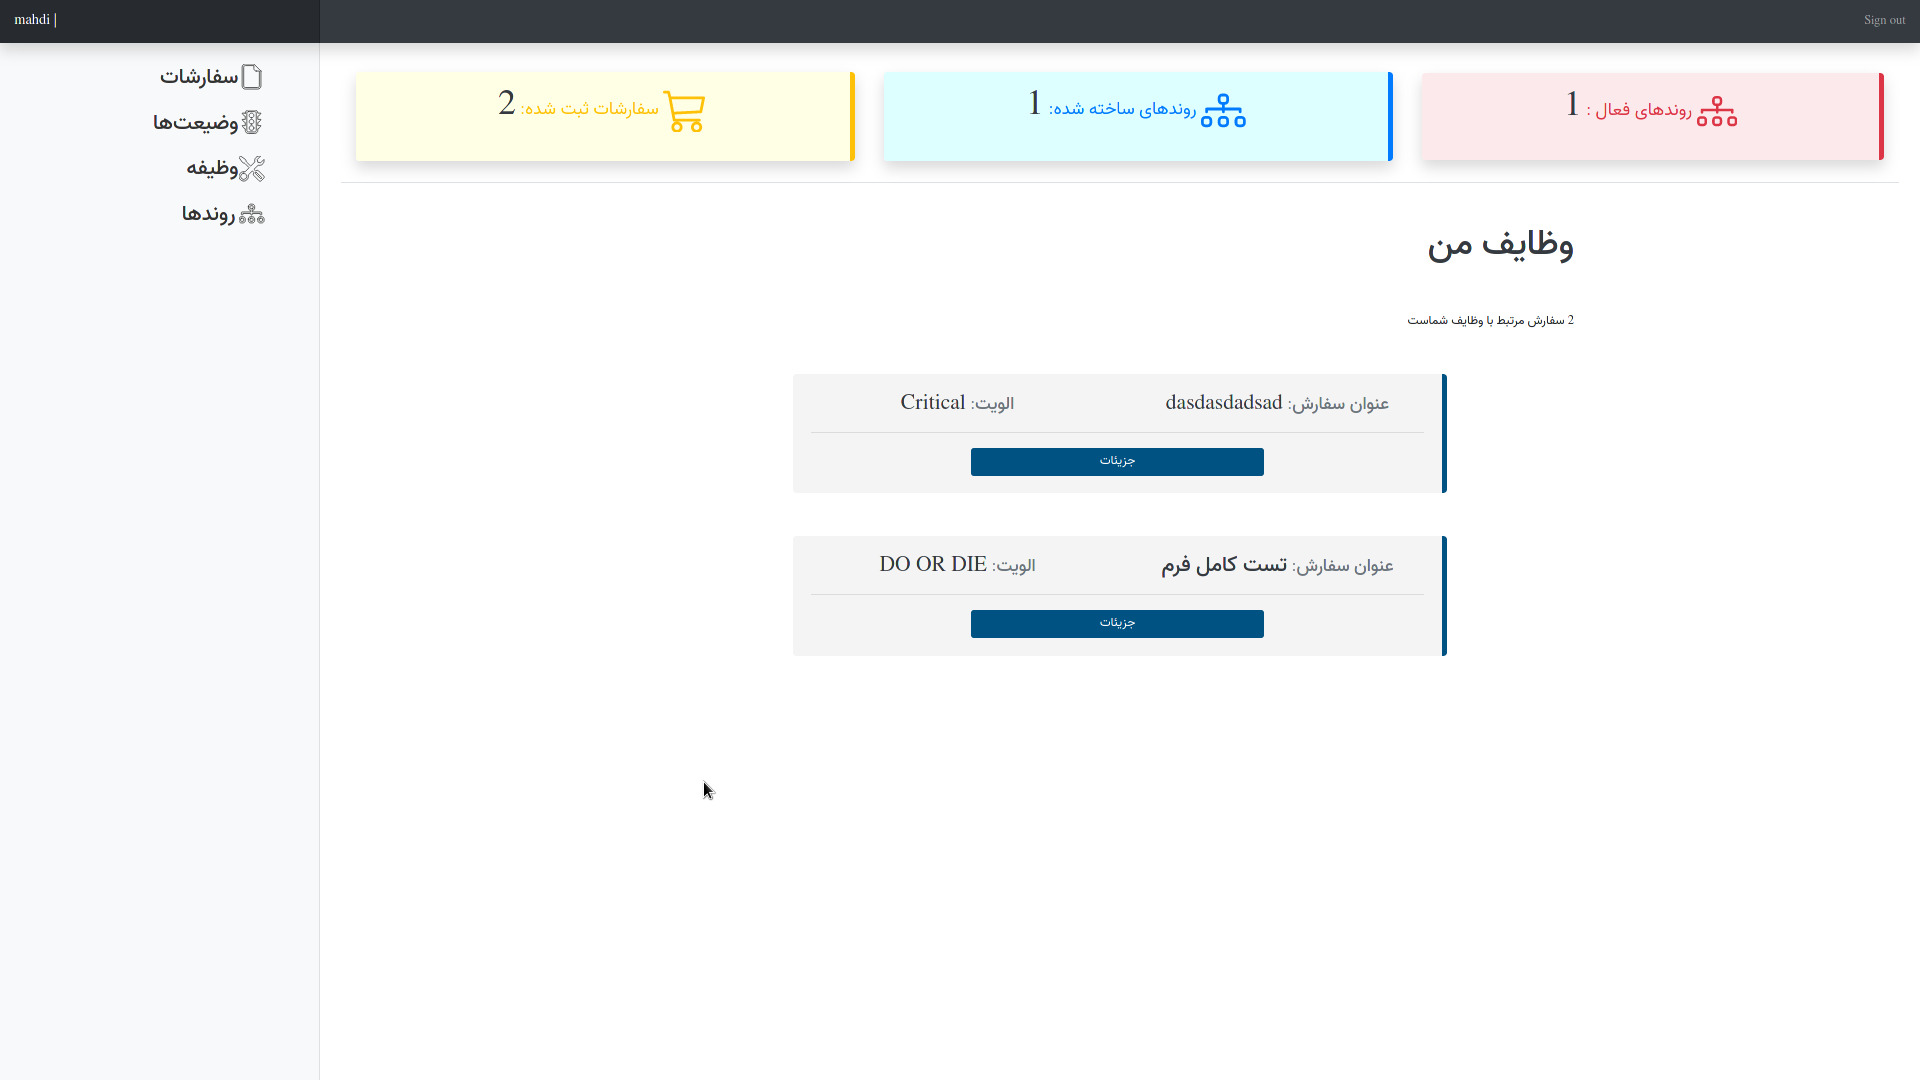
\includegraphics[width=.9\linewidth]{./img/dashboard.png}
\end{center}

\subsection{وضعیت‌ها}
\label{sec:org3f06379}
در بخش وضعیت‌ها میتون لیست وضعیت‌های ساخته شده مشاهده کرد، هر کدام از این وضعیت‌ها دارای امکاناتی مانند
اصلاح و حذف هستند. با استفاده از دکمه ``اضافه کردن'' می‌توان وضعیتی جدید را به وجود آورد.

\begin{center}
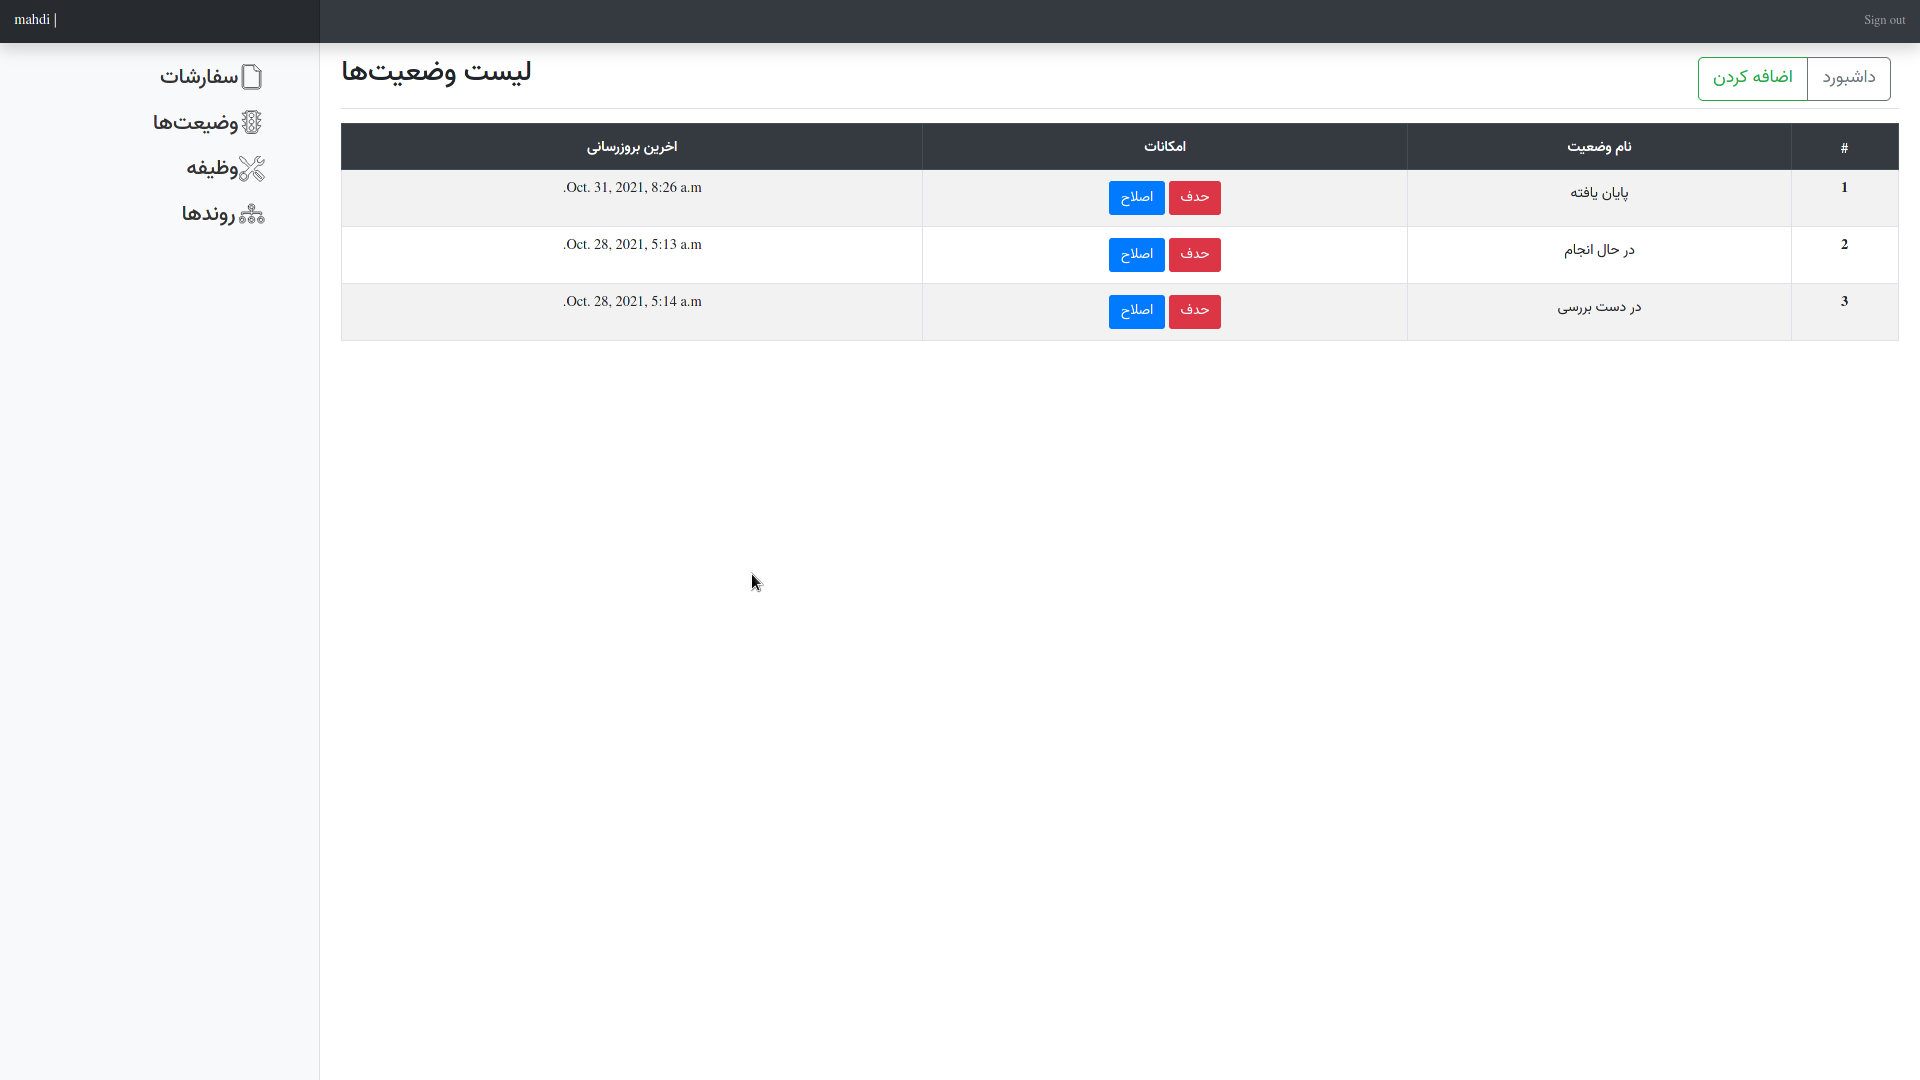
\includegraphics[width=.9\linewidth]{./img/Status.png}
\end{center}

\subsection{وظیفه}
\label{sec:org9d291af}
\subsubsection{لیست وظایف}
\label{sec:orga37dacf}
ظایف شامل عملیات‌هایی هستند که داخل روند‌ها وجود دارند و از انجایی که این عملیات به افراد ابلاغ می‌شوند آن‌ها را وظیفه صدا میزنیم.
در صفحه وظایف می‌توان لیستی از وظایف ساخته شده همراه با جزئیات آن‌ها دید که شامل نام، توضیحات، افراد دارای مجوز و امکاناتی از قبیل اصلاح و حذف دارند.

\begin{center}
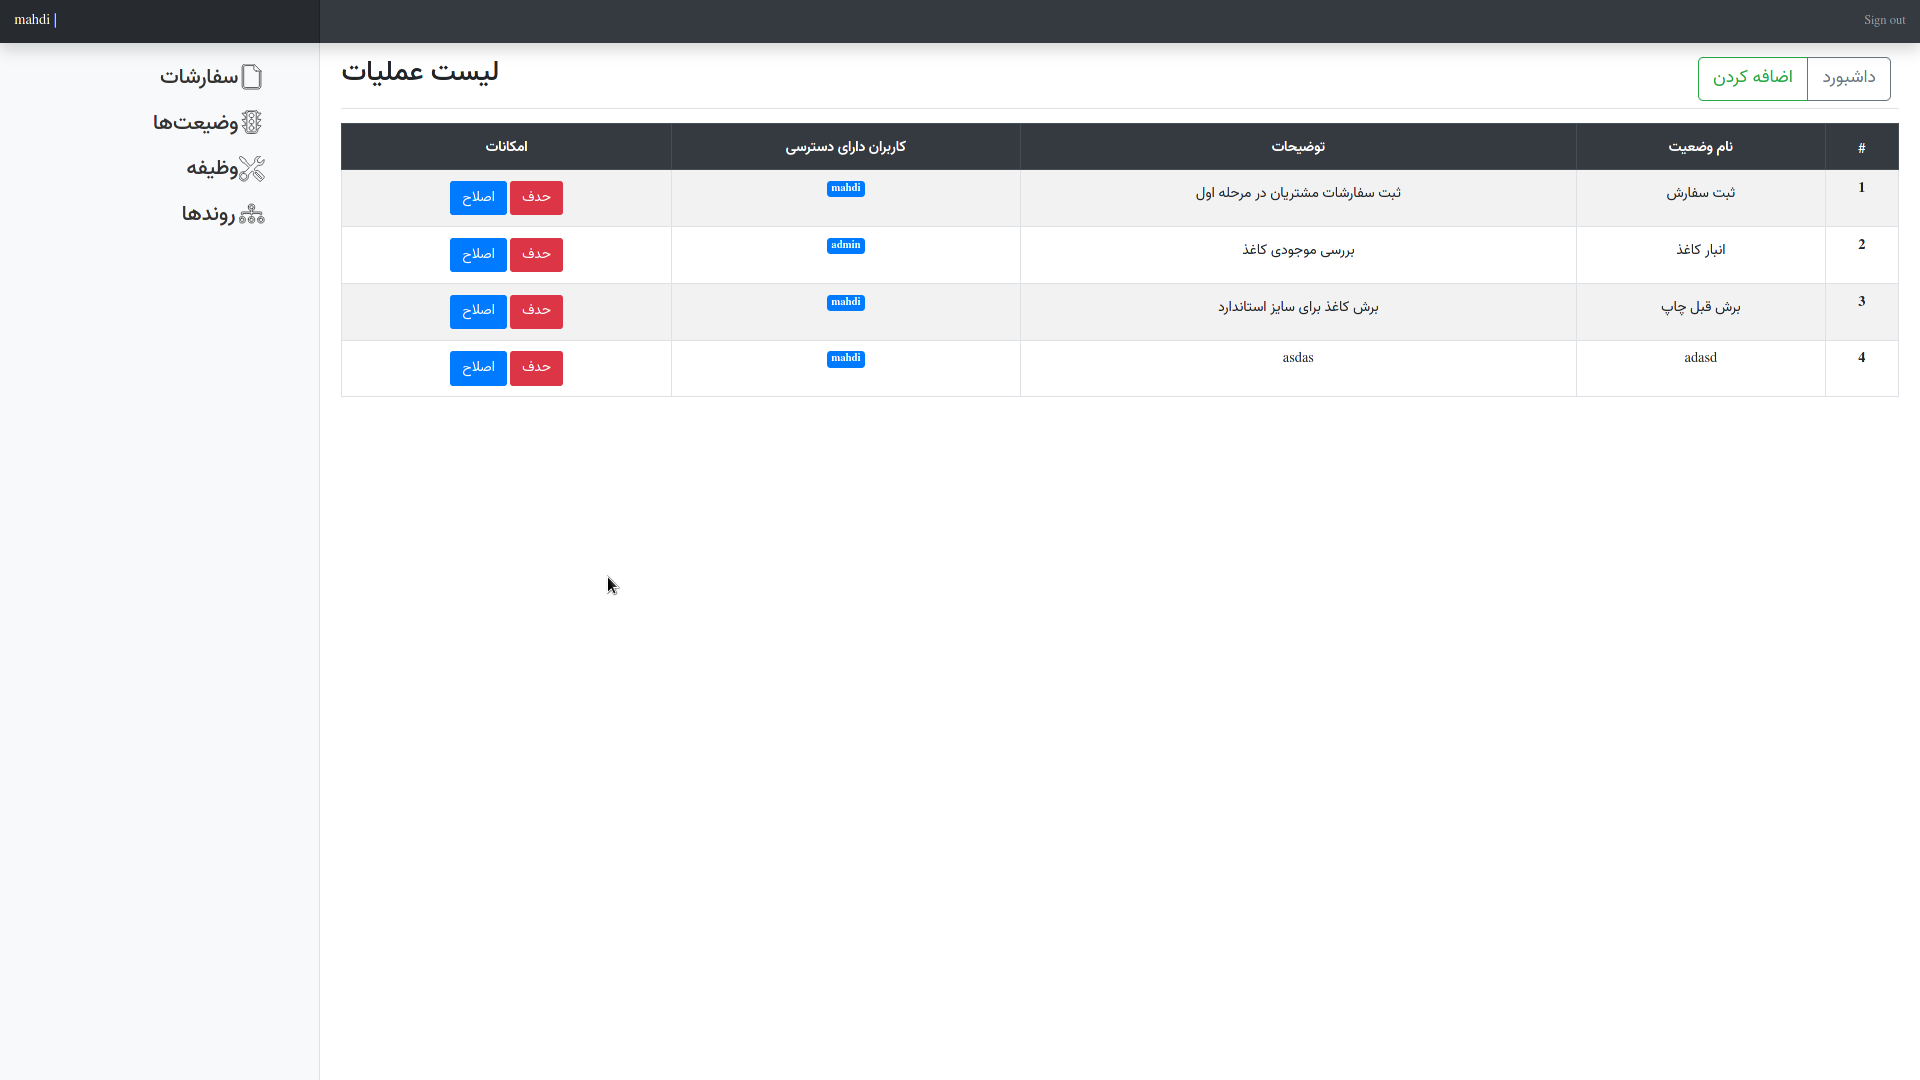
\includegraphics[width=.9\linewidth]{./img/actions.png}
\end{center}

\subsubsection{ساخت وظیفه}
\label{sec:org430605a}
در هنگام تعریف یک وظیفه می‌توانید افراد خاصی که جز کاربران اصلی(غیر از مشتران) هستند را به هر وظیفه به صورت جداگانه اضافه کنید. به صورت پیش فرض امکان خالی گذاشتن این فیلد وجود ندارد و دست کم یک نفر باید به آن‌ها دسترسی داشته باشد. به علاوه در هنگاه اصلاح هم می‌تواند وظیفه‌ای را از کابری سلب کنید یا کاربر دیگری را به آن وظیفه اضافه کنید.

\begin{center}
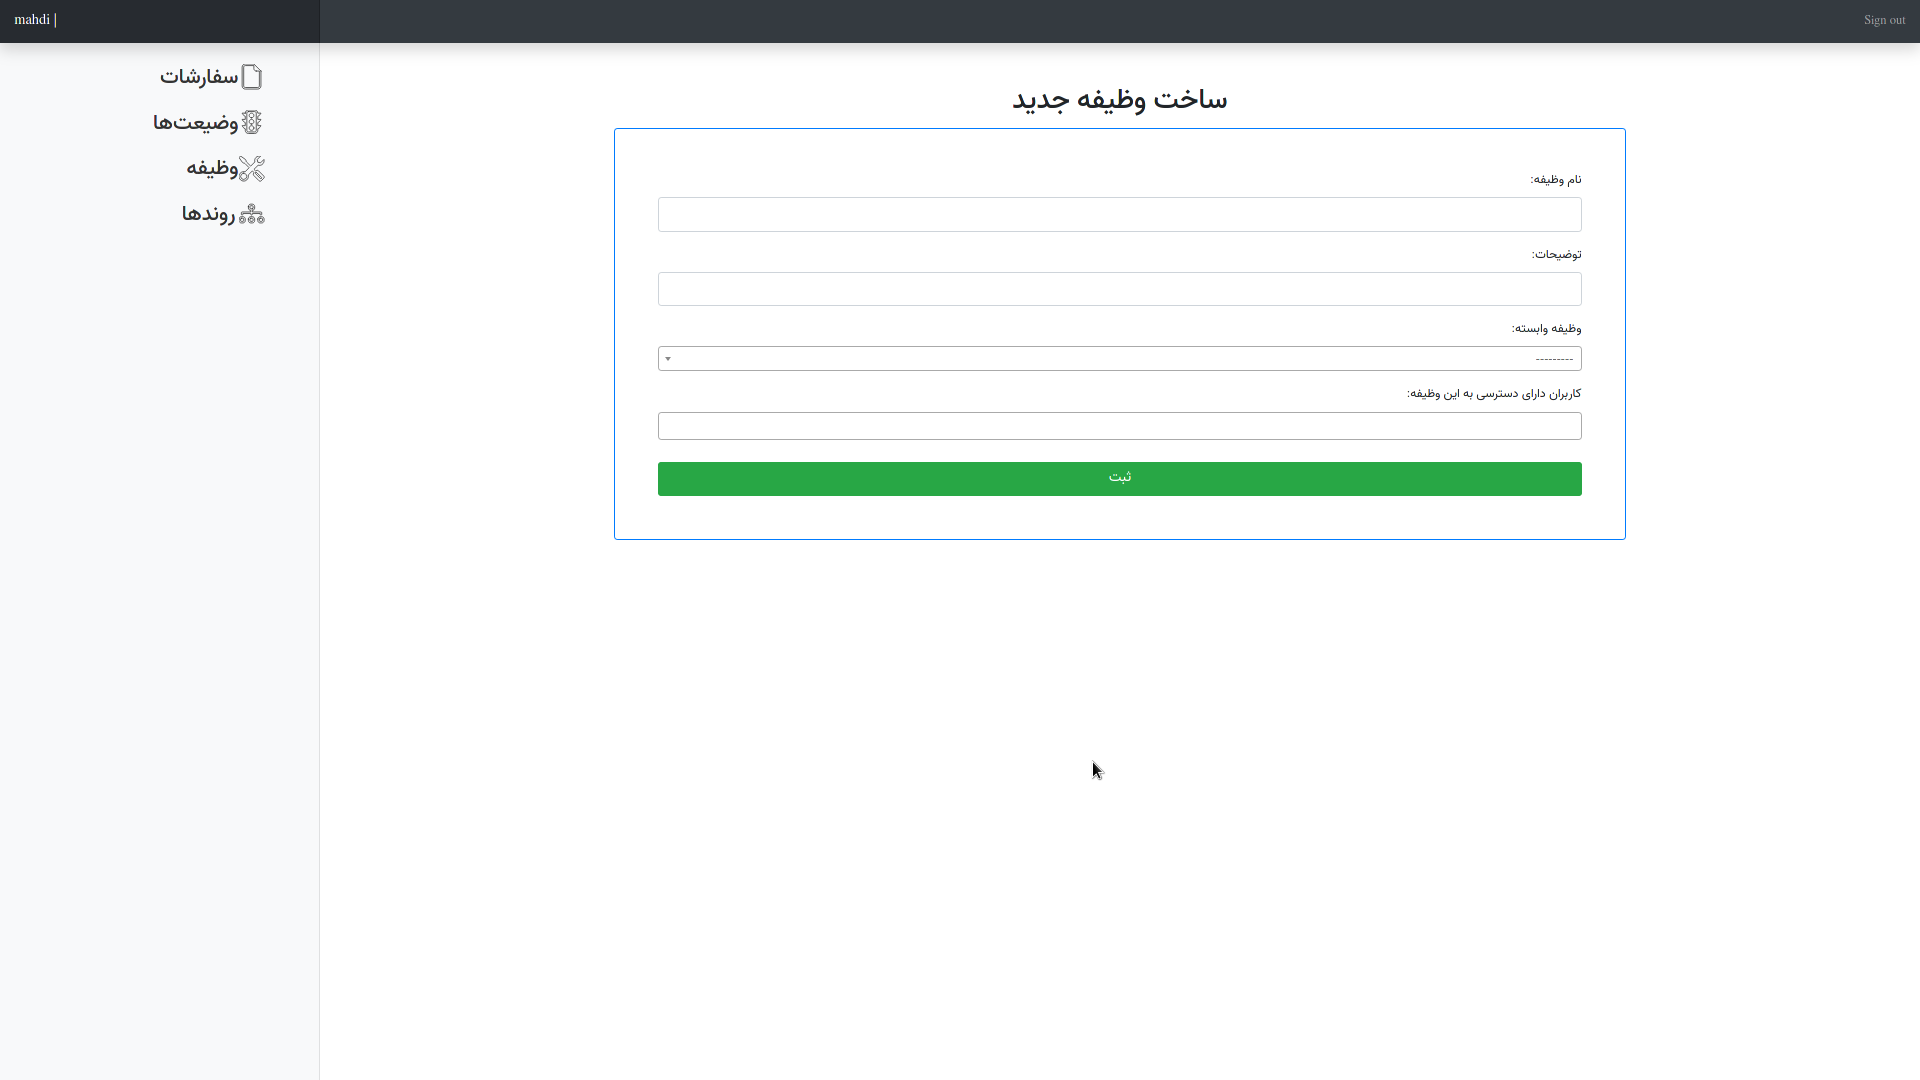
\includegraphics[width=.9\linewidth]{./img/create-action.png}
\end{center}

\subsection{روندها}
\label{sec:org59e1b3c}
در صفحه اصلی روندها هم مانند دیگر صفحات لیستی نمایش داده می‌شود که شامل روندهای ساخته شده هستند و هر ردیف از این لیست اطلاعاتی شامل نام روند، توضیحات روند، وضعیت روند که فعال یا غیر فعال بودن آن را نمایش می‌دهد.

\begin{center}
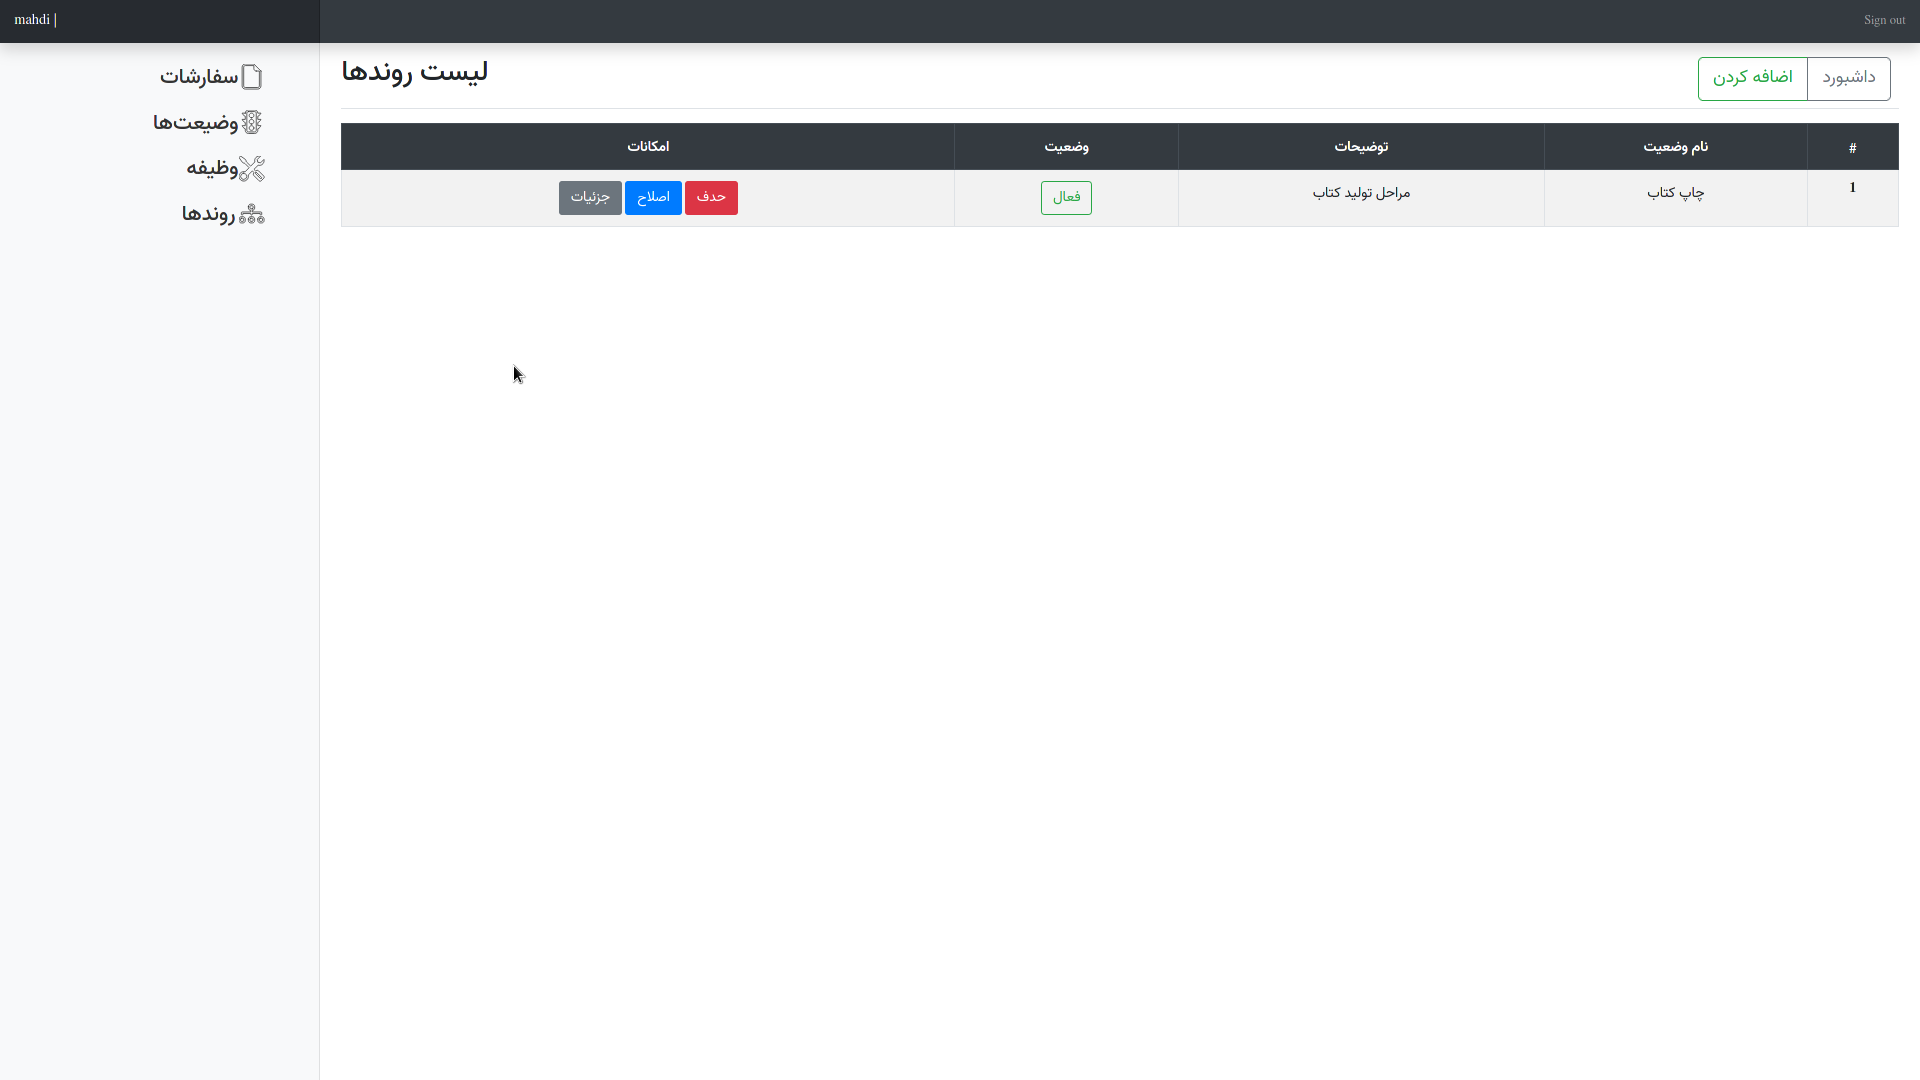
\includegraphics[width=.9\linewidth]{./img/process.png}
\end{center}
\end{document}
